% Backup slides (after \appendix, not counted in the talk).

% ------------------------------------------------------------------------------
\begin{frame}[fragile]{Backup: where the template shortcut comes from}
  \begin{columns}[T]
    \begin{column}{0.42\textwidth}
      \textbf{bad unit}\\[1pt]
\begin{lstlisting}[style=unit]
void sym_0() {
  char *data = NULL;
  data = (char *)malloc(100);
  if (data == NULL) exit(-1);
  strcpy(data, "A String");
  printLine(data);
  ;                  /* no free */
}
\end{lstlisting}
      {\small Function names renamed to \texttt{sym\_N}; abridged.}
    \end{column}
    \begin{column}{0.54\textwidth}
      \textbf{good unit (Original)}\\[1pt]
\begin{lstlisting}[style=unit]
(*\hlc{static void}*) sym_1() {        /* G2B */
  char *data = (char *)ALLOCA(100);
  strcpy(data, "A String"); printLine(data);
}
(*\hlc{static void}*) sym_2() {        /* B2G */
  char *data = (char *)malloc(100);
  ...; printLine(data); free(data);
}
void sym_0() { sym_1(); sym_2(); }
\end{lstlisting}
      {\small Length, function count and \code{static} reveal the label.}
    \end{column}
  \end{columns}
\end{frame}

% ------------------------------------------------------------------------------
\begin{frame}{Backup: task and data}
  \begin{itemize}
    \item One Juliet CWE-401 unit (C or C++) $\to$ leak / no leak
    \item 1,658 bad/good groups, 42 families, 48 flow variants
    \item C 868 / C++ 790 groups; 3,316 units per layer
    \item Debiased G2B / B2G good units $\approx$ 50/50 per flow category
    \item Dev 330 groups (9 variants); eval 1,328 groups (39 variants)
  \end{itemize}
\end{frame}

% ------------------------------------------------------------------------------
\begin{frame}{Backup: Original vs Debiased, all detectors}
  \centering
  {\footnotesize\renewcommand{\arraystretch}{0.86}% generated by figures/make_figures.py -- do not edit
\begin{tabular}{@{}lrr@{}}
\toprule
Detector & Original & Debiased \\
\midrule
\alert{\code{static void} $\Rightarrow$ good (probe)} & \alert{1.000} & \alert{0.333} \\
DeepSeek L1 & 0.961$^\dagger$ & 0.995 \\
Jev L1 & 0.956 & 0.971 \\
\textcolor{NeutDraw}{ASan/LSan (ref.)} & \textcolor{NeutDraw}{0.945} & \textcolor{NeutDraw}{0.945} \\
LoRA decision model L1 & 0.943 & 0.984 \\
\alert{grep: no \code{free}/\code{delete} $\Rightarrow$ leak} & \alert{0.935} & \alert{0.701} \\
Clang SA & 0.822 & 0.855 \\
CodeQL & 0.785 & 0.882 \\
Infer & 0.770 & 0.815 \\
Intern-Decision L1 & 0.642 & 0.825 \\
Qwen3.5-4B L1 & 0.572 & 0.754 \\
Cppcheck & 0.467 & 0.493 \\
LineVul & 0.356 & 0.501 \\
\bottomrule
\end{tabular}
}\\[2pt]
  {\scriptsize Macro-F1 on the eval set (2,656 units). $^\dagger$\,DeepSeek: nested25 subset (664 units).\par}
\end{frame}

% ------------------------------------------------------------------------------
\begin{frame}{Backup: method matrix with versions}
  \footnotesize
  \renewcommand{\arraystretch}{0.9}
  \begin{tabular}{@{}lll@{}}
    \toprule
    Group & Method & Program-analysis idea \\
    \midrule
    Static & grep: is there a \code{free}/\code{delete}? & lexical baseline \\
           & Cppcheck 2.22 & intraprocedural dataflow \\
           & Clang SA 23.1.6 & path-sensitive symbolic execution \\
           & CodeQL 2.27.5 & Datalog-style queries over dataflow \\
           & Infer 1.3 (Pulse) & interprocedural summaries \\
    Learned & LineVul, zero-shot & token classifier (CodeBERT) \\
    Generative & DeepSeek V4.1 Flash (API) $\times$ L1--L4 & L4: LLM facts + Datalog \\
        & Qwen3.5-4B (local) $\times$ L1--L4 & same prompts, one RTX 3090 \\
    Decision & Jev 1.14 (API), Intern-Decision-4B $\times$ L1--L3 & read the option probability \\
             & \textbf{ours}: LoRA decision model $\times$ \{L1, L3\} & fine-tuned score, 3-fold CV \\
    \midrule
    \textcolor{NeutDraw}{Reference} & \textcolor{NeutDraw}{ASan/LSan, Valgrind, Dynamic-enhanced} &
      \textcolor{NeutDraw}{runs the program: shown, not ranked} \\
    \bottomrule
  \end{tabular}
  \vfill
  {\scriptsize Missing output, timeout or compile error counts as a wrong prediction.\par}
\end{frame}

% ------------------------------------------------------------------------------
\begin{frame}{Backup: prompt strategies L1--L4}
  \begin{description}[L4]
    \item[L1] direct: code $\to$ \code{\{label, confidence\}}
    \item[L2] few-shot: + fixed dev examples
    \item[L3] analysis-guided: + Clang SA warnings
    \item[L4] neuro-symbolic: the LLM lists heap facts, \textbf{Datalog} decides
  \end{description}
  \vspace{4pt}
  \centering
  \begin{tikzpicture}[node distance=4mm and 4mm]
    \node[box] (code) {unit\\code};
    \node[hero, right=of code] (llm) {LLM\\{\scriptsize DeepSeek / Qwen3.5-4B}};
    \node[data, right=6mm of llm, font=\scriptsize, align=left] (facts) {%
      \texttt{alloc realloc free}\\
      \texttt{assign pass ret call}\\
      \texttt{global dead(line)}};
    \node[hero, right=of facts] (dl) {Souffl\'e\\{\scriptsize \texttt{leak.dl}}};
    \node[warn, right=of dl] (out) {\texttt{leak(o,\,why)}\\{\scriptsize non-empty $\Rightarrow$ leak}};
    \draw[arr] (code) -- (llm);
    \draw[arr] (llm) -- node[lbl, above] {JSON} (facts);
    \draw[arr] (facts) -- (dl);
    \draw[arr] (dl) -- (out);
  \end{tikzpicture}
  \vfill
  {\scriptsize Same prompt text for DeepSeek and Qwen3.5-4B; temperature 0, thinking off; prompts frozen before eval.
  Decision models read P(leak) for L1--L3.\par}
\end{frame}

% ------------------------------------------------------------------------------
\begin{frame}[fragile]{Backup: L4 (LLM facts + Datalog) is the most robust prompt}
  \begin{columns}[T]
    \begin{column}{0.59\textwidth}
\begin{lstlisting}[style=dl]
reach("main").
reach(g) :- reach(f), call(f, g, l), !dead(l).
new_obj(o, v, f) :- alloc(o, v, f, l),
                    reach(f), !dead(l).
pts(s, v, o) :- new_obj(o, v, f),
                scope(f, v, s).
pts(sd, d, o) :- assign(d, x, f, l), !dead(l),
                 ..., pts(sx, x, o).
freed(o) :- free(v, f, l), reach(f), !dead(l),
            ..., pts(s, v, o).
(*\textcolor{OIblue}{\bfseries leak(o, "never\_freed")}*) :-
        new_obj(o, _, _), !freed(o).
\end{lstlisting}
      {\tiny Abridged from \texttt{juliet\_full/llm/l4/leak.dl} (v3): Andersen-style, flow-insensitive;
      + \texttt{realloc\_fail} rule.\par}
    \end{column}
    \begin{column}{0.39\textwidth}
      \begin{itemize}\small
        \item DeepSeek L4, Debiased: \res{deepseek_L4-layer1}{macro} (L1 \res{deepseek_L1-layer1}{macro})
        \item DeadFree $\Delta$ \res{deepseek_L4-layer3}{d}, smallest of L1--L4 (L1 \res{deepseek_L1-layer3}{d})
        \item FP/FN: L1 \res{deepseek_L1-layer3}{fp}/\res{deepseek_L1-layer3}{fn},
              L4 \res{deepseek_L4-layer3}{fp}/\res{deepseek_L4-layer3}{fn}
        \item 99.87\% of facts grounded to a source line
        \item Qwen3.5-4B L4: \res{qwen_L4-layer1}{macro} $\to$ \res{qwen_L4-layer3}{macro}
      \end{itemize}
    \end{column}
  \end{columns}
  \vfill
  {\scriptsize Paired on nested25 (664 units). A dead \code{free} is dropped by \code{!dead(l)}, so the leak survives.\par}
\end{frame}

% ------------------------------------------------------------------------------
\begin{frame}{Backup: one 4B base model, three uses}
  \centering
  \begin{tikzpicture}[node distance=3mm and 12mm]
    \node[hero, minimum height=16mm, minimum width=22mm] (m) {\textbf{Qwen3.5-4B}\\{\scriptsize same base}};
    \node[box, right=of m, minimum width=62mm, align=left] (u2) {\textbf{read-out}: P(Yes) vs P(No), no generation\\
      {\scriptsize Intern-Decision (same base); plain Qwen3.5-4B as ablation}};
    \node[box, above=of u2, minimum width=62mm, align=left] (u1) {\textbf{generate}: answers L1--L4\\
      {\scriptsize JSON label, or facts for L4}};
    \node[data, below=of u2, minimum width=62mm, align=left] (u3) {\textbf{fine-tune}: LoRA decision model (ours)\\
      {\scriptsize $s=\ell_{\text{Yes}}-\ell_{\text{No}}$; balanced CE + bad$>$good ranking loss}};
    \draw[arr] (m.east) -- (u1.west);
    \draw[arr] (m.east) -- (u2.west);
    \draw[arr] (m.east) -- (u3.west);
  \end{tikzpicture}
  \vspace{4pt}

  {\small LoRA r16, $\alpha$32: 32.5\,M trainable = 0.70\%. Train on two folds, predict the third; merged adapters.\par}
\end{frame}

% ------------------------------------------------------------------------------
\begin{frame}{Backup: Debiased, all methods and strategies}
  \centering
  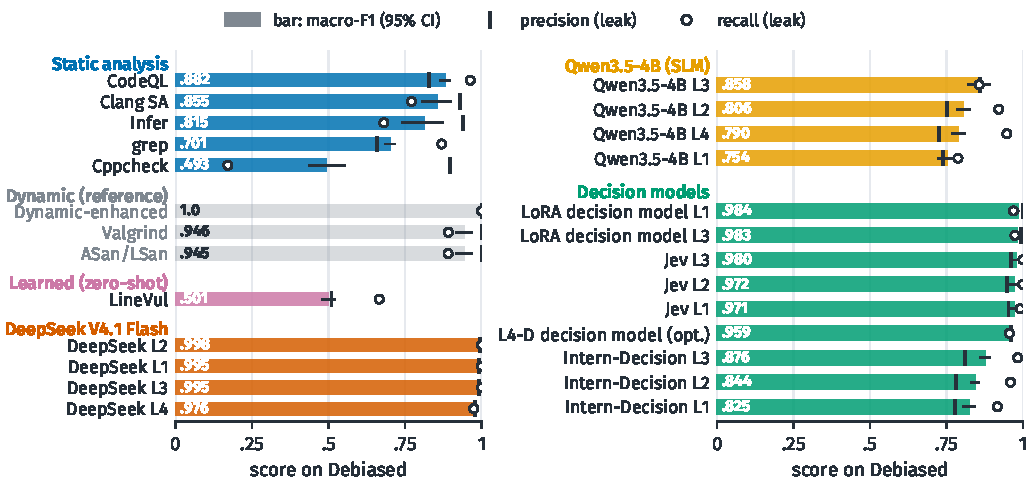
\includegraphics[width=\linewidth,height=0.86\textheight,keepaspectratio]{figures/prf1_full.pdf}
\end{frame}

% ------------------------------------------------------------------------------
% src: McNemar rows from report/final_en/tables/res_mcnemar.tex (18 pre-registered tests, Holm);
%   bootstrap rows from parent analysis juliet_full/analysis/near_llm_bootstrap.py (seed 20261123, B=2000, family-cluster, macro-F1 difference).
\begin{frame}{Backup: paired tests on Debiased (2,656 units)}
  \centering
  \small
  \begin{tabular}{@{}llr@{}}
    \toprule
    A vs B & statistic & result \\
    \midrule
    LoRA L1 vs DeepSeek L1 & $\Delta$macro-F1, 95\% CI & $-0.0113$ $[-0.0143, -0.0084]$ \\
    & only-right units & 12 vs 42 \\
    LoRA L1 vs Jev L1 & $\Delta$macro-F1, 95\% CI & $+0.0132$ $[+0.0029, +0.0282]$ \\
    Intern-Decision L1 vs Qwen3.5-4B L1 & $\Delta$macro-F1 & $+0.0711$ \\
    \midrule
    DeepSeek L1 vs DeepSeek L4 & McNemar $b$/$c$, $p_\text{Holm}$ & 63 / 12, $6.2{\times}10^{-8}$ \\
    DeepSeek L1 vs Qwen3.5-4B L1 & McNemar $b$/$c$, $p_\text{Holm}$ & 641 / 0, $9.4{\times}10^{-140}$ \\
    DeepSeek L2 vs CodeQL & McNemar $b$/$c$, $p_\text{Holm}$ & 306 / 0, $5.7{\times}10^{-67}$ \\
    \bottomrule
  \end{tabular}
  \vfill
  {\scriptsize Bootstrap: 2,000 family-cluster resamples. McNemar: 18 pre-registered tests, Holm-corrected.\par}
\end{frame}

% ------------------------------------------------------------------------------
\begin{frame}{Backup: DeadFree vs Placebo, all methods and strategies}
  \centering
  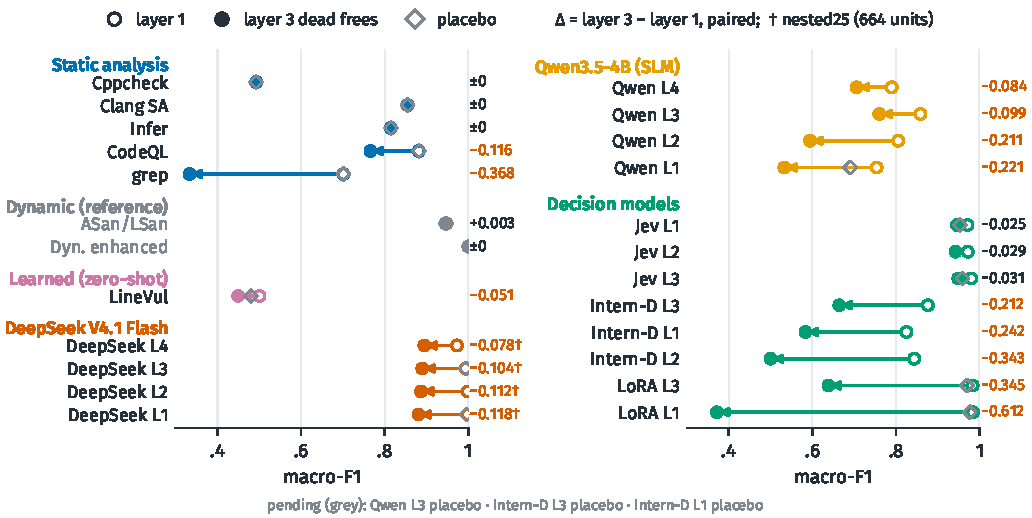
\includegraphics[width=\linewidth,height=0.83\textheight,keepaspectratio]{figures/robustness_full.pdf}
\end{frame}

% ------------------------------------------------------------------------------
\begin{frame}{Backup: DeadFree vs Placebo deltas, key methods}
  \centering
  \small
  \begin{tabular}{@{}lccccc@{}}
    \toprule
    Method & Debiased & DeadFree & $\Delta$ & Placebo & $\Delta$ \\
    \midrule
    DeepSeek L1$^\dagger$ & \res{deepseek_L1-layer3}{base} & \res{deepseek_L1-layer3}{macro} & \res{deepseek_L1-layer3}{d} & \res{deepseek_L1-placebo}{macro} & \res{deepseek_L1-placebo}{d} \\
    Jev L1 & \res{jev_L1-layer1}{macro} & \res{jev_L1-layer3}{macro} & \res{jev_L1-layer3}{d} & \res{jev_L1-placebo}{macro} & \res{jev_L1-placebo}{d} \\
    Qwen3.5-4B L1 & \res{qwen_L1-layer1}{macro} & \res{qwen_L1-layer3}{macro} & \res{qwen_L1-layer3}{d} & \res{qwen_L1-placebo}{macro} & \res{qwen_L1-placebo}{d} \\
    Intern-Decision L1 & \res{intern_L1-layer1}{macro} & \res{intern_L1-layer3}{macro} & \res{intern_L1-layer3}{d} & \res{intern_L1-placebo}{macro} & \res{intern_L1-placebo}{d} \\
    LoRA decision model L1 & \res{lora_L1-layer1}{macro} & \res{lora_L1-layer3}{macro} & \res{lora_L1-layer3}{d} & \res{lora_L1-placebo}{macro} & \res{lora_L1-placebo}{d} \\
    LoRA decision model L3 & \res{lora_L3-layer1}{macro} & \res{lora_L3-layer3}{macro} & \res{lora_L3-layer3}{d} & \res{lora_L3-placebo}{macro} & \res{lora_L3-placebo}{d} \\
    CodeQL & \res{codeql-layer1}{macro} & \res{codeql-layer3}{macro} & \res{codeql-layer3}{d} & \res{codeql-placebo}{macro} & \res{codeql-placebo}{d} \\
    grep & \res{grep-layer1}{macro} & \res{grep-layer3}{macro} & \res{grep-layer3}{d} & \res{grep-placebo}{macro} & \res{grep-placebo}{d} \\
    \bottomrule
  \end{tabular}
  \vfill
  {\scriptsize Macro-F1, paired units. $^\dagger$\,nested25 subset (664 units) for DeadFree and Placebo.\par}
\end{frame}

% ------------------------------------------------------------------------------
\begin{frame}{Backup: where each method fails, by flow category}
  \centering
  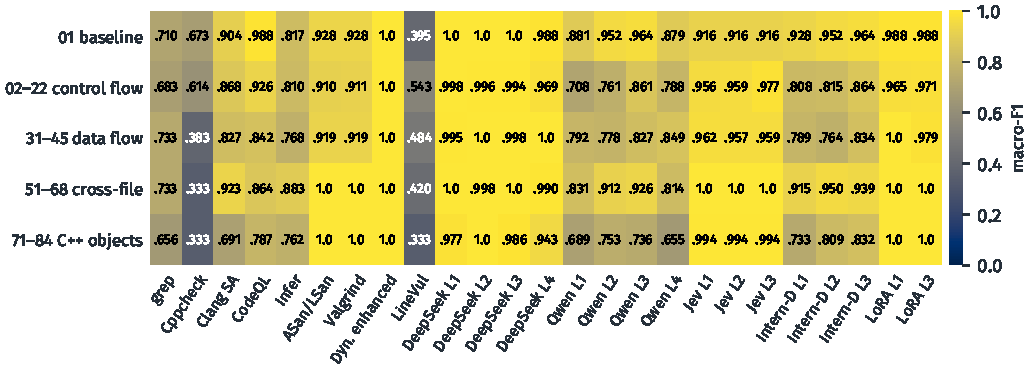
\includegraphics[width=\linewidth,height=0.76\textheight,keepaspectratio]{figures/heatmap.pdf}
  \\[2pt]{\scriptsize Macro-F1 on Debiased, eval set, per Juliet flow-variant group.\par}
\end{frame}

% ------------------------------------------------------------------------------
\begin{frame}{Backup: by leak mechanism and good-unit kind}
  \centering
  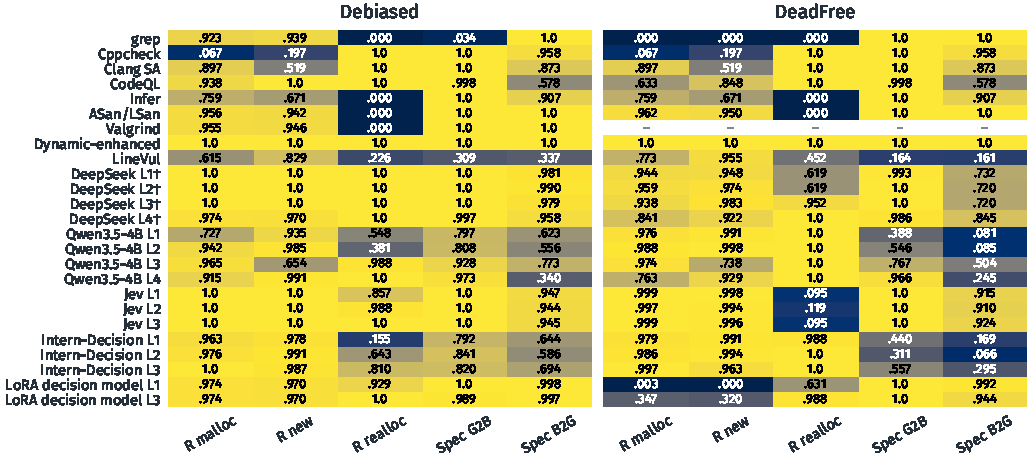
\includegraphics[width=\linewidth,height=0.80\textheight,keepaspectratio]{figures/mechanism.pdf}
  \\[2pt]{\scriptsize Leak recall per mechanism (bad units); specificity per good kind (G2B / B2G). Debiased vs DeadFree.\par}
\end{frame}

% ------------------------------------------------------------------------------
\begin{frame}{Backup: repeat agreement and merged vs unmerged LoRA}
  \begin{columns}[T]
    \begin{column}{0.48\textwidth}
      {\small Same prompt, 3 runs (Debiased)\\[2pt]
      % generated by figures/make_figures.py -- do not edit
\begin{tabular}{@{}lrr@{}}
\toprule
Model & units & all 3 runs agree \\
\midrule
DeepSeek L1 & 200 & 1.000 \\
DeepSeek L2 & 200 & 1.000 \\
DeepSeek L3 & 200 & 0.990 \\
Jev L1 & 2,656 & 0.989 \\
Jev L2 & 2,656 & 0.996 \\
Jev L3 & 2,656 & 0.995 \\
Qwen L1 & & \textit{pending} \\
Qwen L2 & & \textit{pending} \\
Qwen L3 & & \textit{pending} \\
\bottomrule
\end{tabular}
\par}
    \end{column}
    \begin{column}{0.48\textwidth}
      \begin{itemize}\small
        \item Reported LoRA = adapters \textbf{merged} into BF16 weights
        \item Unmerged, Debiased: L1 \res{lora_unmerged_L1-layer1}{macro}, L3 \res{lora_unmerged_L3-layer1}{macro}
        \item Predictions that differ: \res{x}{unmerged_flips_L1} (L1), \res{x}{unmerged_flips_L3} (L3) of 2,656
        \item Only BF16 rounding of large logits
      \end{itemize}
    \end{column}
  \end{columns}
\end{frame}

% ------------------------------------------------------------------------------
\begin{frame}{Backup: CodeQL batching artifact}
  \begin{itemize}
    \item CodeQL builds one database per \textbf{50 units} (7.36\,s $\to$ 0.32\,s per unit)
    \item \code{\_08} units define helpers \code{staticReturnsTrue/False}, not renamed per unit
    \item In a shared database the guard cannot be resolved: ``may not be freed'' fires
    \item \textbf{4} extra false positives on eval good units (per-unit runs are clean)
    \item Not corrected: configuration frozen before eval
  \end{itemize}
\end{frame}

% ------------------------------------------------------------------------------
\begin{frame}{Backup: cost of every API run}
  \begin{columns}[T]
    \begin{column}{0.60\textwidth}
      {\scriptsize\resizebox{\linewidth}{!}{% generated by figures/make_figures.py from juliet_full/llm/ledger.jsonl
\begin{tabular}{@{}llrr@{}}
\toprule
Provider & Runs & calls & cost \\
\midrule
DeepSeek & Debiased (incl.\ dev, repeats, latency) & 13,877 & \textyen5.46 \\
DeepSeek & DeadFree & 11,824 & \textyen5.37 \\
DeepSeek & Placebo & 1,328 & \textyen0.42 \\
DeepSeek & Original & 664 & \textyen0.30 \\
DeepSeek & demo & 30 & \textyen0.01 \\
\textbf{DeepSeek} & \textbf{total} & \textbf{27,723} & \textbf{\textyen11.57} \\
\midrule
Jev & Debiased (incl.\ dev, repeats, latency) & 27,420 & \$1.23 \\
Jev & DeadFree & 8,868 & \$0.42 \\
Jev & Placebo & 5,312 & \$0.20 \\
Jev & Original & 2,656 & \$0.10 \\
Jev & demo & 11 & \$0.00 \\
\textbf{Jev} & \textbf{total} & \textbf{44,267} & \textbf{\$1.95} \\
\bottomrule
\end{tabular}
}\par}
    \end{column}
    \begin{column}{0.37\textwidth}
      \begin{itemize}\small
        \item DeepSeek cap \textyen10; hard stop at \textyen9.5
        \item Total: \textyen\res{x}{cost_deepseek} and \$\res{x}{cost_jev}
        \item Per 1k units: DeepSeek L1 \textyen0.397, Jev L1 \$0.0345
        \item Hence DeepSeek nested25 (664 units)
        \item Local models: no API cost
      \end{itemize}
    \end{column}
  \end{columns}
  % src: per-1k cost from report/final_en/generated/numbers.tex (res-x-cost1k_deepseek_L1, res-x-cost1k_jev_L1)
\end{frame}

% ------------------------------------------------------------------------------
\begin{frame}{Backup: latency at concurrency 1}
  \centering
  {\tiny\renewcommand{\arraystretch}{0.92}\resizebox{\linewidth}{!}{% generated by figures/make_figures.py from figures/latency_c1.csv
\begin{tabular}{@{}lrl@{}}
\toprule
Method & s / unit & Source (juliet\_full/\ldots); note \\
\midrule
grep & <0.001 & \texttt{static/results/grep\_v0/layer1/lat300\_c1.jsonl}; median of 300 units (1 µs) \\
Cppcheck & 0.008 & \texttt{static\_stage2.md}; lat300 per unit \\
Clang SA & 0.018 & \texttt{static\_stage2.md}; lat300 per unit \\
Infer & 0.278 & \texttt{static\_stage2.md}; lat300 per unit \\
CodeQL & 7.36 & \texttt{static\_stage2.md}; per unit: database creation + queries (20 units) \\
CodeQL (50 per database) & 0.318 & \texttt{static\_stage2.md}; 50 units per database; amortized (hollow marker) \\
LineVul (GPU) & 0.006 & \texttt{gpu\_stage1.md}; GPU (RTX 3090) \\
LineVul (CPU) & 0.088 & \texttt{gpu/results/linevul\_cpu/layer1/lat300\_cpu\_quiet.jsonl}; CPU 6 threads; quiet; median of 300 \\
DeepSeek L1 & 0.721 & \texttt{llm\_stage2b.md}; lat300\_c1\_L1 at load ~21; quiet 0.640 s on 30 dev units (llm\_stage2a) \\
Qwen L1 & 0.665 & \texttt{gpu\_stage1.md}; vLLM from dell; 30 requests \\
Jev L1 & 0.961 & \texttt{llm\_stage2b.md}; lat300\_c1\_L1 at load ~22 \\
Intern-D L1 & 0.083 & \texttt{gpu\_stage1.md}; /decide read-out from dell (82.7 ms) \\
LoRA L1 & 0.105 & \texttt{decision\_ft\_stage2.md}; latency300; dell end-to-end \\
LoRA L3 & 0.133 & \texttt{decision\_ft\_stage2.md}; latency300; dell end-to-end \\
ASan/LSan & 0.134 & \texttt{data\_stage4.md}; lat300\_c1; compile included \\
Valgrind & 0.407 & \texttt{data\_stage4.md}; lat300\_c1; compile included \\
Dyn. enhanced & 1.194 & \texttt{data\_stage4.md}; lat300\_c1; compile included \\
\bottomrule
\end{tabular}
}\par}
  \vfill
  {\scriptsize Median end-to-end per unit. Source table: \texttt{figures/latency\_c1.csv}.\par}
\end{frame}

% ------------------------------------------------------------------------------
\begin{frame}{Backup: are the labels still right? Compile and run every unit}
  \begin{columns}[T]
    \begin{column}{0.46\textwidth}
      \begin{itemize}\small
        \item gcc and clang compile \textbf{3,316 / 3,316} units in every layer
        \item No good unit flagged by ASan/LSan or Dynamic-enhanced
        \item Labels never changed; disagreements explained
      \end{itemize}
    \end{column}
    \begin{column}{0.51\textwidth}
      {\footnotesize Dynamic-enhanced: what it takes to catch the 1,658 bad units\\[2pt]
      \begin{tabular}{@{}lr@{}}
        \toprule
        Needed & units \\
        \midrule
        plain run, every seed & 1,448 \\
        some seeds only (variant 12, random) & 34 \\
        \texttt{use\_globals=0} (globals at exit) & 68 \\
        \texttt{realloc} failure injected & 108 \\
        \bottomrule
      \end{tabular}}
    \end{column}
  \end{columns}
\end{frame}

% ------------------------------------------------------------------------------
\begin{frame}{Backup: why dynamic tools are a reference line, not a competitor}
  \begin{itemize}
    \item Plain ASan/LSan: precision 1.000, macro-F1 \res{asan_lsan-layer1}{macro} on Debiased
    \item Misses: \code{realloc} failure 0/84; globals at exit; random branch not taken
    \item LSan with \code{use\_stacks=0}: default options miss 175 more bad units
    \item Dynamic-enhanced reaches \res{dynamic_enhanced-layer1}{macro}: we chose inputs and faults
    \item They need a build, a run and the right input
  \end{itemize}
\end{frame}

% ------------------------------------------------------------------------------
\begin{frame}{Backup: demo dry run (stage unit, all detectors)}
  \centering
  {\small% generated by figures/make_figures.py from presentation/demo/recordings/stage_final_v2.json
\begin{tabular}{@{}lccc r@{}}
\toprule
Detector & bad & good twin & bad + dead free & ms \\
\midrule
grep & \cmark\,leak & \cmark\,no leak & \xmark\,no leak\,\textcolor{OIvermil}{\small flipped} & 2 \\
Clang SA & \cmark\,leak & \cmark\,no leak & \cmark\,leak & 191 \\
old LoRA L1 (unit labels) & \cmark\,leak & \cmark\,no leak & \xmark\,no leak\,\textcolor{OIvermil}{\small flipped} & 378 \\
old LoRA L3 (unit labels) & \cmark\,leak & \cmark\,no leak & \xmark\,no leak\,\textcolor{OIvermil}{\small flipped} & 760 \\
FT L4-D (opt.) & \cmark\,leak & \cmark\,no leak & \cmark\,leak & 223 \\
DeepSeek L1 & \cmark\,leak & \cmark\,no leak & \cmark\,leak & 887 \\
DeepSeek L3 & \cmark\,leak & \cmark\,no leak & \cmark\,leak & 1209 \\
Jev L1 & \cmark\,leak & \cmark\,no leak & \cmark\,leak & 948 \\
\bottomrule
\end{tabular}
\par}
  \vfill
  {\scriptsize Fallback: \texttt{demo.py --replay recordings/stage\_final.json} or \texttt{recordings/stage\_final.mp4}.
  Dry-run cost: \textyen\res{x}{demo_cny} DeepSeek, \$\res{x}{demo_usd} Jev.\par}
\end{frame}

% ------------------------------------------------------------------------------
\begin{frame}{Backup: earlier SecVulEval study}
  \begin{itemize}
    \item Real CVE functions from SecVulEval (Ahmed et al., AIware'26)
    \item Pair task: MiMo single-order accuracy 86.7\%
    \item Swapped order: MiMo 74.44\%, DeepSeek 61.67\%
    \item Same lesson: check the benchmark before ranking models
  \end{itemize}
\end{frame}

% ------------------------------------------------------------------------------
% generated by figures/make_figures.py -- do not edit (input outside a frame)
\begin{frame}{Backup: result files used (1/5)}
\centering
{\tiny\renewcommand{\arraystretch}{0.85}\setlength{\tabcolsep}{4pt}\begin{tabular}{@{}llll@{}}
\toprule
Method & Layer & Run file (juliet\_full/\ldots; r = results) & sha256 \\
\midrule
grep & Debiased & \texttt{static/r/grep\_v0/layer1/full\_v1.jsonl} & \texttt{9a425c0e} \\
grep & DeadFree & \texttt{static/r/grep\_v0/layer3/full\_v1.jsonl} & \texttt{a0a26ccd} \\
grep & Placebo & \texttt{static/r/grep\_v0/placebo/full\_v1.jsonl} & \texttt{0e7c92ed} \\
grep & Original & \texttt{static/r/grep\_v0/original/full\_v1.jsonl} & \texttt{5c3bf9ea} \\
Cppcheck & Debiased & \texttt{static/r/cppcheck/layer1/full\_v2.jsonl} & \texttt{b3ae0a0e} \\
Cppcheck & DeadFree & \texttt{static/r/cppcheck/layer3/full\_v1.jsonl} & \texttt{3bd521e3} \\
Cppcheck & Placebo & \texttt{static/r/cppcheck/placebo/full\_v1.jsonl} & \texttt{aade3fed} \\
Cppcheck & Original & \texttt{static/r/cppcheck/original/full\_v1.jsonl} & \texttt{26245ae1} \\
Clang SA & Debiased & \texttt{static/r/clang\_sa/layer1/full\_v2.jsonl} & \texttt{9fff5bc7} \\
Clang SA & DeadFree & \texttt{static/r/clang\_sa/layer3/full\_v1.jsonl} & \texttt{29c2c3cb} \\
Clang SA & Placebo & \texttt{static/r/clang\_sa/placebo/full\_v1.jsonl} & \texttt{a031bf11} \\
Clang SA & Original & \texttt{static/r/clang\_sa/original/full\_v1.jsonl} & \texttt{d48a49c1} \\
CodeQL & Debiased & \texttt{static/r/codeql/layer1/full\_batch50\_merged.jsonl} & \texttt{1e41db0c} \\
CodeQL & DeadFree & \texttt{static/r/codeql/layer3/full\_batch50.jsonl} & \texttt{26cf528a} \\
CodeQL & Placebo & \texttt{static/r/codeql/placebo/full\_batch50.jsonl} & \texttt{203de4f7} \\
CodeQL & Original & \texttt{static/r/codeql/original/full\_batch50.jsonl} & \texttt{e6133458} \\
Infer & Debiased & \texttt{static/r/infer/layer1/full\_per\_file\_merged.jsonl} & \texttt{ba59f70d} \\
Infer & DeadFree & \texttt{static/r/infer/layer3/full\_per\_file.jsonl} & \texttt{69dda662} \\
Infer & Placebo & \texttt{static/r/infer/placebo/full\_per\_file.jsonl} & \texttt{161f789c} \\
Infer & Original & \texttt{static/r/infer/original/full\_per\_file.jsonl} & \texttt{36074229} \\
LineVul & Debiased & \texttt{gpu/r/linevul\_gpu/layer1/deveval\_v1.jsonl} & \texttt{8bc1535e} \\
LineVul & DeadFree & \texttt{gpu/r/linevul\_gpu/layer3/all\_v1.jsonl} & \texttt{2bf0d6ab} \\
\bottomrule
\end{tabular}\par}
\vfill
{\scriptsize Scored with \texttt{juliet\_full/analysis/score.py} on the eval set (2,656 units); \texttt{figures/make\_figures.py}.\par}
\end{frame}
\begin{frame}{Backup: result files used (2/5)}
\centering
{\tiny\renewcommand{\arraystretch}{0.85}\setlength{\tabcolsep}{4pt}\begin{tabular}{@{}llll@{}}
\toprule
Method & Layer & Run file (juliet\_full/\ldots; r = results) & sha256 \\
\midrule
LineVul & Placebo & \texttt{gpu/r/linevul\_gpu/placebo/all\_v1.jsonl} & \texttt{19529812} \\
LineVul & Original & \texttt{gpu/r/linevul\_gpu/original/all\_v1.jsonl} & \texttt{7d2e9b26} \\
ASan/LSan & Debiased & \texttt{data/r/asan\_lsan/layer1/full\_v1.jsonl} & \texttt{684c4195} \\
ASan/LSan & DeadFree & \texttt{data/r/asan\_lsan/stress/full\_v1.jsonl} & \texttt{97a9eb40} \\
ASan/LSan & Placebo & \texttt{data/r/asan\_lsan/placebo/full\_v1.jsonl} & \texttt{9eda685e} \\
ASan/LSan & Original & \texttt{data/r/asan\_lsan/original/full\_v1.jsonl} & \texttt{8945394e} \\
Valgrind & Debiased & \texttt{data/r/valgrind/layer1/full\_v1.jsonl} & \texttt{fb6481b7} \\
Dynamic-enhanced & Debiased & \texttt{data/r/dynamic\_enhanced/layer1/full\_v1.jsonl} & \texttt{758daeac} \\
Dynamic-enhanced & DeadFree & \texttt{data/r/dynamic\_enhanced/stress/full\_v1.jsonl} & \texttt{cf47c76c} \\
Dynamic-enhanced & Placebo & \texttt{data/r/dynamic\_enhanced/placebo/full\_v1.jsonl} & \texttt{181e81b2} \\
DeepSeek L1 & Debiased & \texttt{llm/r/deepseek\_flash/layer1/eval\_L1\_r1.jsonl} & \texttt{912db2f0} \\
DeepSeek L1 & DeadFree & \texttt{llm/r/deepseek\_flash/layer3/l3\_n25\_L1\_r1.jsonl} & \texttt{376d1393} \\
DeepSeek L1 & Placebo & \texttt{llm/r/deepseek\_flash/placebo/pl\_n25\_L1\_r1.jsonl} & \texttt{6480450e} \\
DeepSeek L1 & Original & \texttt{llm/r/deepseek\_flash/original/orig\_n25\_L1\_r1.jsonl} & \texttt{034fdebe} \\
DeepSeek L2 & Debiased & \texttt{llm/r/deepseek\_flash/layer1/eval\_L2\_r1.jsonl} & \texttt{ee6c51f4} \\
DeepSeek L2 & DeadFree & \texttt{llm/r/deepseek\_flash/layer3/l3\_n25\_L2\_r1.jsonl} & \texttt{369a2a1f} \\
DeepSeek L3 & Debiased & \texttt{llm/r/deepseek\_flash/layer1/eval\_L3\_r1.jsonl} & \texttt{4bf6db11} \\
DeepSeek L3 & DeadFree & \texttt{llm/r/deepseek\_flash/layer3/l3\_n25\_L3\_r1.jsonl} & \texttt{6f396914} \\
DeepSeek L3 & Placebo & \texttt{llm/r/deepseek\_flash/placebo/pl\_n25\_L3\_r1.jsonl} & \texttt{c56b0f67} \\
DeepSeek L4 & Debiased & \texttt{llm/r/deepseek\_flash/layer1/eval\_L4\_r1.jsonl} & \texttt{0af89897} \\
DeepSeek L4 & DeadFree & \texttt{llm/r/deepseek\_flash/layer3/l3\_n25\_L4\_r1.jsonl} & \texttt{37d32759} \\
Qwen3.5-4B L1 & Debiased & \texttt{llm/r/qwen3\_5\_4b/layer1/eval\_L1\_r1.jsonl} & \texttt{0c952905} \\
\bottomrule
\end{tabular}\par}
\vfill
{\scriptsize Scored with \texttt{juliet\_full/analysis/score.py} on the eval set (2,656 units); \texttt{figures/make\_figures.py}.\par}
\end{frame}
\begin{frame}{Backup: result files used (3/5)}
\centering
{\tiny\renewcommand{\arraystretch}{0.85}\setlength{\tabcolsep}{4pt}\begin{tabular}{@{}llll@{}}
\toprule
Method & Layer & Run file (juliet\_full/\ldots; r = results) & sha256 \\
\midrule
Qwen3.5-4B L1 & DeadFree & \texttt{llm/r/qwen3\_5\_4b/layer3/l3\_eval\_L1\_r1.jsonl} & \texttt{c9e21163} \\
Qwen3.5-4B L1 & Placebo & \texttt{llm/r/qwen3\_5\_4b/placebo/pl\_eval\_L1\_r1.jsonl} & \texttt{41998d19} \\
Qwen3.5-4B L1 & Original & \texttt{llm/r/qwen3\_5\_4b/original/orig\_eval\_L1\_r1.jsonl} & \texttt{d0a08dbd} \\
Qwen3.5-4B L2 & Debiased & \texttt{llm/r/qwen3\_5\_4b/layer1/eval\_L2\_r1.jsonl} & \texttt{43c641b2} \\
Qwen3.5-4B L2 & DeadFree & \texttt{llm/r/qwen3\_5\_4b/layer3/l3\_eval\_L2\_r1.jsonl} & \texttt{337dc906} \\
Qwen3.5-4B L3 & Debiased & \texttt{llm/r/qwen3\_5\_4b/layer1/eval\_L3\_r1.jsonl} & \texttt{d0d1469a} \\
Qwen3.5-4B L3 & DeadFree & \texttt{llm/r/qwen3\_5\_4b/layer3/l3\_eval\_L3\_r1.jsonl} & \texttt{3c3ddd18} \\
Qwen3.5-4B L3 & Placebo & \texttt{llm/r/qwen3\_5\_4b/placebo/pl\_eval\_L3\_r1.jsonl} & \texttt{9fdeb3fd} \\
Qwen3.5-4B L4 & Debiased & \texttt{llm/r/qwen3\_5\_4b/layer1/eval\_L4\_r1.jsonl} & \texttt{266a3cc9} \\
Qwen3.5-4B L4 & DeadFree & \texttt{llm/r/qwen3\_5\_4b/layer3/l3\_eval\_L4\_r1.jsonl} & \texttt{5c2708a1} \\
Jev L1 & Debiased & \texttt{llm/r/jev/layer1/eval\_L1\_r1.jsonl} & \texttt{b0a4576e} \\
Jev L1 & DeadFree & \texttt{llm/r/jev/layer3/l3\_eval\_L1\_r1.jsonl} & \texttt{59fe6079} \\
Jev L1 & Placebo & \texttt{llm/r/jev/placebo/pl\_eval\_L1\_r1.jsonl} & \texttt{77d9bfce} \\
Jev L1 & Original & \texttt{llm/r/jev/original/orig\_eval\_L1\_r1.jsonl} & \texttt{6d574be5} \\
Jev L2 & Debiased & \texttt{llm/r/jev/layer1/eval\_L2\_r1.jsonl} & \texttt{ca0bf9e1} \\
Jev L2 & DeadFree & \texttt{llm/r/jev/layer3/l3\_eval\_L2\_r1.jsonl} & \texttt{fbe5242d} \\
Jev L3 & Debiased & \texttt{llm/r/jev/layer1/eval\_L3\_r1.jsonl} & \texttt{a5977265} \\
Jev L3 & DeadFree & \texttt{llm/r/jev/layer3/l3\_eval\_L3\_r1.jsonl} & \texttt{cb498e82} \\
Jev L3 & Placebo & \texttt{llm/r/jev/placebo/pl\_eval\_L3\_r1.jsonl} & \texttt{f5c6f04e} \\
Intern-Decision L1 & Debiased & \texttt{gpu/r/intern\_decision/layer1/eval\_L1\_r1.jsonl} & \texttt{f1e87ff7} \\
Intern-Decision L1 & DeadFree & \texttt{gpu/r/intern\_decision/layer3/l3\_eval\_L1\_r1.jsonl} & \texttt{7a52bf2f} \\
Intern-Decision L1 & Placebo & \texttt{gpu/r/intern\_decision/placebo/pl\_eval\_L1\_r1.jsonl} & \texttt{a784841c} \\
\bottomrule
\end{tabular}\par}
\vfill
{\scriptsize Scored with \texttt{juliet\_full/analysis/score.py} on the eval set (2,656 units); \texttt{figures/make\_figures.py}.\par}
\end{frame}
\begin{frame}{Backup: result files used (4/5)}
\centering
{\tiny\renewcommand{\arraystretch}{0.85}\setlength{\tabcolsep}{4pt}\begin{tabular}{@{}llll@{}}
\toprule
Method & Layer & Run file (juliet\_full/\ldots; r = results) & sha256 \\
\midrule
Intern-Decision L1 & Original & \texttt{gpu/r/intern\_decision/original/orig\_eval\_L1\_r1.jsonl} & \texttt{84f4bd18} \\
Intern-Decision L2 & Debiased & \texttt{gpu/r/intern\_decision/layer1/eval\_L2\_r1.jsonl} & \texttt{3feb32b2} \\
Intern-Decision L2 & DeadFree & \texttt{gpu/r/intern\_decision/layer3/l3\_eval\_L2\_r1.jsonl} & \texttt{37419c78} \\
Intern-Decision L3 & Debiased & \texttt{gpu/r/intern\_decision/layer1/eval\_L3\_r1.jsonl} & \texttt{9251594a} \\
Intern-Decision L3 & DeadFree & \texttt{gpu/r/intern\_decision/layer3/l3\_eval\_L3\_r1.jsonl} & \texttt{01ea2eb7} \\
Intern-Decision L3 & Placebo & \texttt{gpu/r/intern\_decision/placebo/pl\_eval\_L3\_r1.jsonl} & \texttt{b5be8128} \\
LoRA decision model L1 & Debiased & \texttt{decision\_ft/r/decision\_ft/layer1/L1\_cv\_v1.jsonl} & \texttt{82f901e2} \\
LoRA decision model L1 & DeadFree & \texttt{decision\_ft/r/decision\_ft/layer3/L1\_cv\_v1.jsonl} & \texttt{797bb4bb} \\
LoRA decision model L1 & Placebo & \texttt{decision\_ft/r/decision\_ft/placebo/L1\_cv\_v1.jsonl} & \texttt{123ddefc} \\
LoRA decision model L1 & Original & \texttt{decision\_ft/r/decision\_ft/original/L1\_cv\_v1.jsonl} & \texttt{3bf56a58} \\
LoRA decision model L3 & Debiased & \texttt{decision\_ft/r/decision\_ft/layer1/L3\_cv\_v1.jsonl} & \texttt{d76d94b9} \\
LoRA decision model L3 & DeadFree & \texttt{decision\_ft/r/decision\_ft/layer3/L3\_cv\_v1.jsonl} & \texttt{903680f7} \\
LoRA decision model L3 & Placebo & \texttt{decision\_ft/r/decision\_ft/placebo/L3\_cv\_v1.jsonl} & \texttt{d52fa746} \\
L4-D decision model (opt.) & Debiased & \texttt{l4d\_ft/r/lora\_l4d\_opt/layer1/eval\_r1\_units.jsonl} & \texttt{87791590} \\
L4-D decision model (opt.) & DeadFree & \texttt{l4d\_ft/r/lora\_l4d\_opt/layer3/eval\_r1\_units.jsonl} & \texttt{3409d5cc} \\
L4-D decision model (opt.) & Placebo & \texttt{l4d\_ft/r/lora\_l4d\_opt/placebo/eval\_r1\_units.jsonl} & \texttt{16edbdfa} \\
L4-D decision model (opt.) & Original & \texttt{l4d\_ft/r/lora\_l4d\_opt/original/eval\_r1\_units.jsonl} & \texttt{206a3089} \\
No-LoRA read-out L1 & Debiased & \texttt{decision\_ft/r/qwen\_readout\_zeroshot/layer1/L1\_v1.jsonl} & \texttt{cac9ab4c} \\
No-LoRA read-out L1 & DeadFree & \texttt{decision\_ft/r/qwen\_readout\_zeroshot/layer3/L1\_v1.jsonl} & \texttt{64ee4b28} \\
LoRA decision model L1 unmerged & Debiased & \texttt{decision\_ft/r/decision\_ft/layer1/unmerged\_L1\_fold0\_v1.jsonl (+2)} & \texttt{23d377ec} \\
No-LoRA read-out L3 & Debiased & \texttt{decision\_ft/r/qwen\_readout\_zeroshot/layer1/L3\_v1.jsonl} & \texttt{72bf7f18} \\
No-LoRA read-out L3 & DeadFree & \texttt{decision\_ft/r/qwen\_readout\_zeroshot/layer3/L3\_v1.jsonl} & \texttt{f738465d} \\
\bottomrule
\end{tabular}\par}
\vfill
{\scriptsize Scored with \texttt{juliet\_full/analysis/score.py} on the eval set (2,656 units); \texttt{figures/make\_figures.py}.\par}
\end{frame}
\begin{frame}{Backup: result files used (5/5)}
\centering
{\tiny\renewcommand{\arraystretch}{0.85}\setlength{\tabcolsep}{4pt}\begin{tabular}{@{}llll@{}}
\toprule
Method & Layer & Run file (juliet\_full/\ldots; r = results) & sha256 \\
\midrule
LoRA decision model L3 unmerged & Debiased & \texttt{decision\_ft/r/decision\_ft/layer1/unmerged\_L3\_fold0\_v1.jsonl (+2)} & \texttt{0ed06f4f} \\
\bottomrule
\end{tabular}\par}
\vfill
{\scriptsize Scored with \texttt{juliet\_full/analysis/score.py} on the eval set (2,656 units); \texttt{figures/make\_figures.py}.\par}
\end{frame}

